\documentclass[11pt]{article}
\usepackage{mathtools}
\usepackage{mdframed}
\usepackage{fullpage}
\usepackage{amsfonts}
\usepackage{tikz}            % if you delete this, you will have trouble with the included picture. You can delete the picture.
\usetikzlibrary{automata, positioning}


%edit this for each class
\newcommand\name{John Vincent} %%%%%%%%%%%%%%  WRITE YOUR NAME HERE
\newcommand\classname{COMS 331}
\newcommand\assignment{homework 1}



\newcounter{excounter}
\setcounter{excounter}{1}
\newcommand\question[2]{\vskip 1em  \noindent\textbf{\arabic{excounter}\addtocounter{excounter}{1}:} \emph{#1} \noindent#2}


% You can also erase this if you do not have package hancyhdr
% Fancy footnote.........
\usepackage{fancyhdr}  %% If it does not work with your latex installation, you may just delete this...
\pagestyle{fancy}
\usepackage{lastpage}
\rfoot{\name, page \thepage/\pageref{LastPage}}
\cfoot{}
\rhead{}
\lhead{}
\renewcommand{\headrulewidth}{0pt}
\renewcommand{\footrulewidth}{0pt}
\DeclarePairedDelimiter\ceil{\lceil}{\rceil}
\DeclarePairedDelimiter\floor{\lfloor}{\rfloor}



\begin{document}


  {\bf \classname \hspace{1cm} \assignment\hfill \name}
  \vskip 2em


  \question{}
  $b^*(a^{*}c^{+}b^{*})^{*}a^{*}$

  \question{}
  $(a+(bb)+c)^*$

  \question{}
  $(a+b+c)^*$\\
  this language is any string that contains the letters a, b, and c in any order
  of any length

  \question{}
  $(a+b)^*c^*(a+b)^*$\\
  the expression can not be simplified, the language consist of strings that
  have any amount and any order of a's and b's followed by any amount of c's
  followed again by and amount and any order of a's and b's

  \question{}

  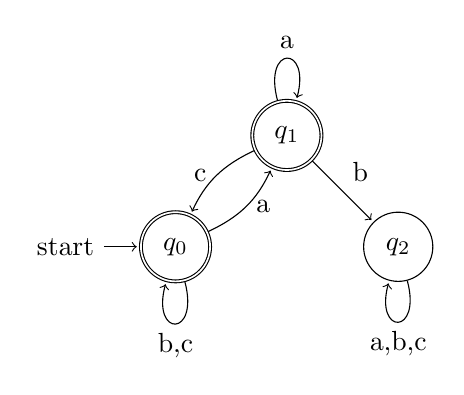
\begin{tikzpicture}[shorten >=1pt,node distance=2cm,on grid,auto]
   \node[state,initial,accepting] (q_0)   {$q_0$};
   \node[state,accepting] (q_1) [above right=of q_0] {$q_1$};
   \node[state](q_2) [below right=of q_1] {$q_2$};
    \path[->]
    (q_0) edge [bend right=20] node [right] {a} (q_1)
          edge [loop below] node {b,c} ()
    (q_1) edge node  {b} (q_2)
          edge [loop above] node {a} ()
          edge [bend right=20] node [left] {c} (q_0)
    (q_2) edge [loop below] node {a,b,c} ();
\end{tikzpicture}

\question{}

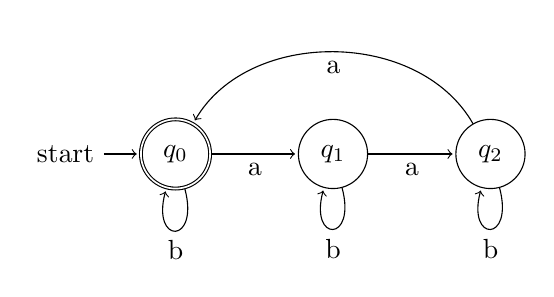
\begin{tikzpicture}[shorten >=1pt,node distance=2cm,on grid,auto]
 \node[state,initial,accepting] (q_0)   {$q_0$};
 \node[state] (q_1) [right=of q_0] {$q_1$};
 \node[state](q_2) [right=of q_1] {$q_2$};
  \path[->]
  (q_0) edge node [below] {a} (q_1)
        edge [loop below] node {b} ()
  (q_1) edge node [below] {a} (q_2)
        edge [loop below] node {b} ()
  (q_2) edge [bend right=60] node {a} (q_0)
        edge [loop below] node {b} ();
\end{tikzpicture}


\end{document}
